\section{Preliminaries \& Setup}
\label{sec:methodology}

We consider reinforcement learning with LLMs, where prompts $x$ are sampled from a data distribution $D$. 
Our setup follows a generator–trainer split across GPUs: a subset of GPUs (\emph{generators}) use optimized inference kernels for high-throughput rollout generation, while the remaining GPUs (\emph{trainers}) run the training backend (FSDP) and update parameters. 
We denote by $\pi_{\text{gen}}^\theta$ and $\pi_{\text{train}}^\theta$ the model with parameters $\theta$ on the generator and training backends, respectively. 
For each prompt, the old policy $\pi_{gen}^{\theta_{old}}$ on the generator GPUs produces candidate completions, which are then assigned scalar rewards. 
Policy optimization proceeds by maximizing a clipped surrogate objective, taking expectations over $x \sim D$ and rollouts from $\pi_{gen}^{\theta_{old}}$.


\paragraph{Training Regimen}
All experiments are conducted on the RL for reasoning domain, where the model produces a thinking trace enclosed with special tokens (\texttt{<think>} $\ldots$ \texttt{</think>}) and a final solution. Unless noted, training uses a sequence length of $16,384$ tokens: $12,288$ for thinking, $2,048$ for the solution, and an additional $2,048$ for the input prompt. We adopt the $12,288$ thinking budget for faster iteration, and show in \Cref{sec:diff_axes} that \scalerl\ extrapolations remain predictive when training with larger thinking budgets ($32,768$). For math RL experiments, we use the Polaris-53K dataset~\citep{polaris2025} with a batch size of 768 (48 prompts with 16 generations each). %and a maximum output sequence length of $14,336$ tokens. 
In our setup, scaling RL compute corresponds to running multiple epochs over the training prompts. More details about training, including SFT and hyper-parameters, are in Appendix~\ref{appendix:setup}.


\paragraph{Base RL Algorithm}
As our starting point in \S~\ref{sec:experiments}, we start with a ``base'' algorithm that resembles GRPO~\citep{shao2024deepseekmath} without any KL regularization term, in line with large-scale training reports~\citep{rastogi2025magistral,minimax_m1}. Additionally, we include the asymmetric DAPO clipping~\citep{yu2025dapo}, because of its widespread adoption as a default approach to avoid entropy collapse and maintain output diversity. 

For a given prompt $x$, the old policy $\pi_{\text{gen}}(\theta_{\text{old}})$ generates $G$ candidate completions $\{y_i\}_{i=1}^G$, each assigned a scalar reward $r_i$. 
We compute advantages $\hat{A}_i$ and group-normalized advantages using:
\begin{equation*}
    \hat{A}_i = r_i - \mathrm{mean}(\{r_j\}_{j=1}^G),  \quad
    \hat{A}_i^{G} = \hat{A}_i/(\mathrm{std}(\{r_j\}_{j=1}^G) + \epsilon).
    % \label{eq:advantage}
\end{equation*}
Each completion $y_i$ of length $|y_i|$ contributes at the token-level importance sampling (IS) ratios $\rho_{i,t}(\theta)$, with asymmetric upper and lower clipping thresholds, akin to DAPO~\citep{yu2025dapo}:
\begin{equation}
    \rho_{i,t}(\theta) := \frac{\pi^\theta_{train}(y_{i,t} \mid x, y_{i,<t})}{\pi^{\theta_{\text{old}}}_{gen}(y_{i,t} \mid x, y_{i,<t})} = \frac{\pi^\theta_{train}(y_{i,t})}{\pi^{\theta_{\text{old}}}_{gen}(y_{i,t})}; \quad \mathrm{clip}_{\mathrm{asym}}(\rho, \epsilon^-, \epsilon^+) := \mathrm{clip}(\rho,\, 1-\epsilon^-, 1+\epsilon^+).
    \label{eq:is}
\end{equation}

We aggregate losses at the \emph{sample level}, i.e., averaging per-sample token losses before averaging across samples. 
The surrogate objective is given by:
\begin{equation}\label{eq:grpo_loss}
    \mathcal{J}(\theta) 
    % = \mathbb{E}_{x \sim D,\, \{y_i\}_{i=1}^G \sim \pi_{gen}(\cdot \mid x, \theta_{\text{old}})} 
    = \mathbb{E}_{\begin{subarray}{l} \, x \sim D, \\ \{y_i\}_{i=1}^G \sim {\pi_{\text{gen}}^{\theta_{\text{old}}}(\cdot \mid x)} \end{subarray}}
    \left[ \frac{1}{G} \sum_{i=1}^G \frac{1}{|y_i|} \sum_{t=1}^{|y_i|}
    \min\!\left( \rho_{i,t}(\theta)\hat{A}_i^{G},\; \mathrm{clip_{asym}}(\rho_{i,t}(\theta), \epsilon^-, \epsilon^+)\hat{A}_i^{G} \right) \right].
\end{equation}


\paragraph{Controlling Generation Lengths}  
To prevent reasoning output lengths from exploding during training, which harms training stability and efficiency, we use \textbf{interruptions}~\citep{glm_4.1v,qwen3technicalreport} that forcibly stop overly long generations by appending an end-of-thinking phrase (e.g., `` \texttt{</think>}''), signaling the LLM to terminate its reasoning and produce a final answer. We revisit this choice later in \Cref{sec:loo} and compare it with length-penalty that penalizes long generations~\citep{yu2025dapo,team2025kimi}.
% \looseness=-1




\subsection{Predictive compute-scaling and fitting curves}


Unlike pre-training, which typically uses power-law to fit predictive curves, we model pass rate versus $\log(\text{\emph{compute}})$ with a sigmoidal function (\Cref{eq:sigmoid_law}). We do so because we found the sigmoidal fit to be much more robust and stable compared to power law empirically, which we discuss further in Appendix~\ref{appendix:curve_to_fit}. Moreover, our choice is consistent with prior work that use sigmoid-like power laws to capture bounded metrics such as accuracy~\citep{ruan2024,srivastava2022bigbench}.  



%And we observed similar trend for our validation curves as well, motivating further to use sigmoidal fits. 
% Further discussion on the choice of curve fitting is provided in Appendix~\ref{appendix:curve_to_fit}.

Similar to pre-training studies~\citep{misfitting,porian2025}, we find that excluding the very early low-compute regime yields more stable fits, after which training follows a predictable trajectory. Unless noted otherwise, all our scaling fits begin after $\sim$1.5k GPU hours. Further details of the fitting procedure are provided in Appendix~\ref{appendix:fitting_curves} and the robustness of our curve fitting is discussed in Appendix~\ref{appendix:fits_robustness}. 

\paragraph{Interpreting scaling curves} Intuitively, a sigmoidal curve captures saturating returns - grows slowly in the low-compute regime, accelerates sharply through a mid-range of efficient scaling, and then saturates at high compute. We also provide a schematic interpretation of the parameters $A, B, \text{ and } C_{mid}$ of the sigmoidal curve in \Cref{fig:interpreting_fit}. We see that $B, C_\text{mid}$ primarily affects the efficiency of the run, and $A$ denotes the asymptotic performance at large compute scale. Further discussion of these parameters is provided in Appendix~\ref{appendix:interpreting_fit}.

\paragraph{Scaling curve on held-out validation}
Consistent with pre-training practice~\citep{hoffmann2022training,porian2025}, we measure predictive performance on \textbf{in-distribution} validation data. Since our training runs span multiple epochs, we hold out randomly selected $1,000$ prompts from the Polaris-53k dataset for validation and use the remainder for training. The scaling curves are fitted on the validation points, which measure the average pass rate every $100$ training steps, with $16$ generations per prompt on the $1,000$ held-out prompts. 



\begin{figure}[t]
    \centering
    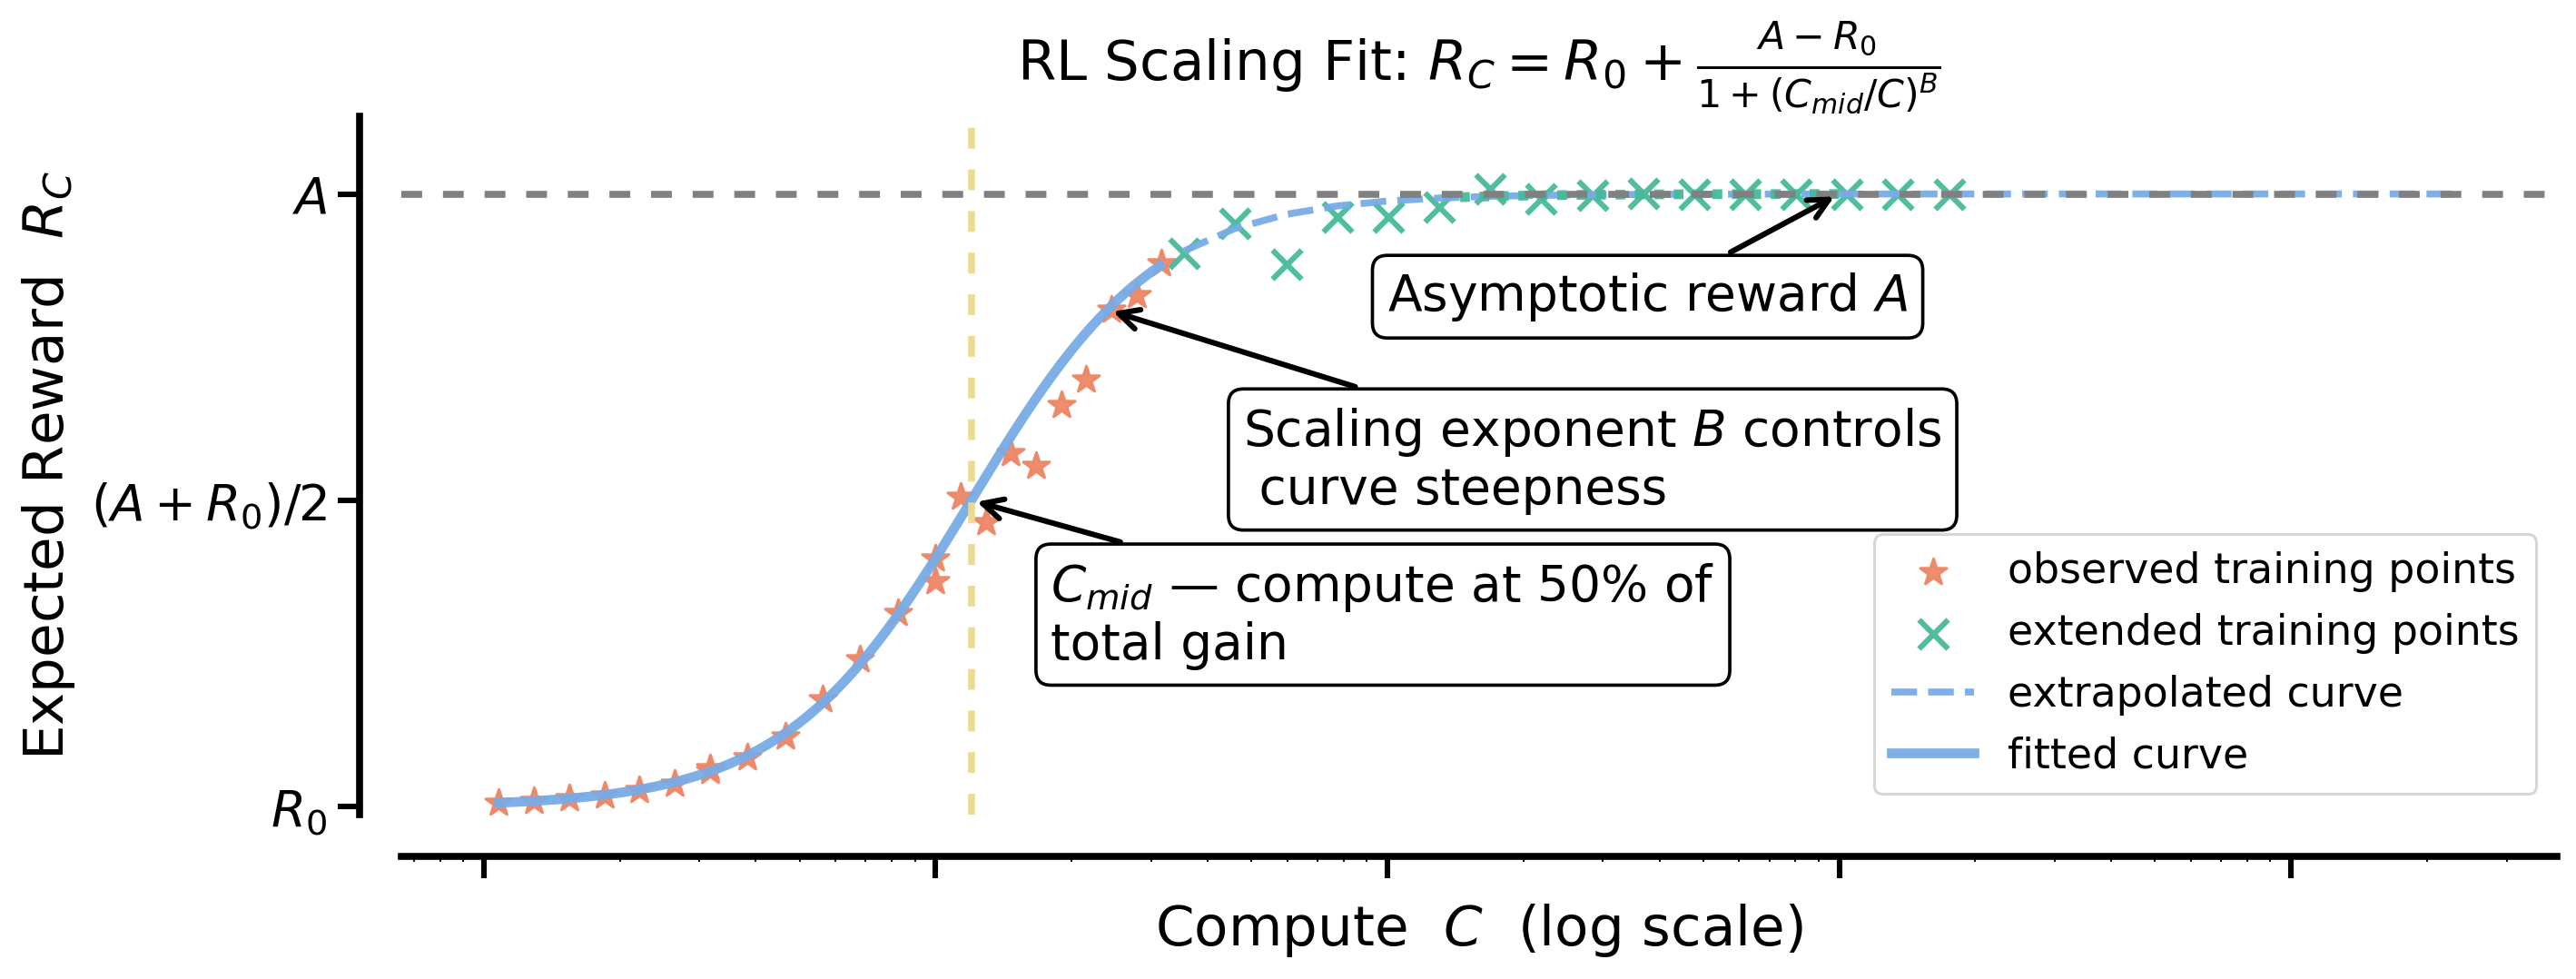
\includegraphics[width=0.8\textwidth]{paper_figs/interpreting_fit.png}
    \caption{
    \small{\textbf{Interpreting \cref{eq:sigmoid_law}}. We provide an example fit illustrating the roles of parameters $A$, $B$, and $C_{\text{mid}}$.
    $C_{\text{mid}}$ determines the compute point at which half of the total gain is achieved - smaller values correspond to faster ascent toward the asymptote.
    $B$ controls the curve’s steepness, with larger values indicating greater efficiency.
    $A$ represents the asymptotic performance reached at large compute scales. Further discussion is provided in Appendix~\ref{appendix:interpreting_fit}.}
    }
    \label{fig:interpreting_fit}
\end{figure}




% \paragraph{Interpreting \cref{eq:sigmoid_law}}
% The parameters $C_{mid}$ and $B$ effect the efficiency of the curve, while parameter $A$ controls the asymptotic performance


 